\chapter{Степени с целым показателем}\markright{Глава 6}
\begin{definition}\term{Степень} (\emph{power}) \(a^{n}\) при натуральном \(n\) — произведение \(n\) одинаковых множителей \(a\).\end{definition}
\begin{definition}\term{Основание степени} (\emph{base}) \(a^{n}\) — число \(a\), которое возводят в степень.\end{definition}
\begin{definition}\term{Показатель степени} (\emph{exponent}) \(a^{n}\) — число \(n\); при натуральном \(n\) оно указывает количество одинаковых множителей \(a\).\end{definition}
\begin{definition}\term{Нулевая степень} (\emph{zeroth power}) ненулевого числа определяется равенством \(a^{0} = 1\).\end{definition}
\begin{definition}\term{Отрицательная целая степень} (\emph{negative integer power}) определяется равенством \(a^{- n} = \frac{1}{a^{n}}\) при \(a \ne  0\) и натуральном \(n\).\end{definition}
\begin{definition}\term{Стандартный вид положительного числа} (\emph{scientific notation}) — \(c \cdot  10^{n}\), где \(1 \le  c < 10\) и \(n\) — целое число.\end{definition}
\section*{Свойства степеней}
При умножении степеней одного основания показатели складывают: \(a^{m} \cdot  a^{n} = a^{m + n}\).\par
При делении показатели вычитают: \(\frac{a^{m}}{a^{n}} = a^{m - n},\allowbreak a \ne  0\).\par
При возведении степени в степень показатели перемножают: \((a^{m})^{n} = a^{mn}\).\par
Степень произведения: \((ab)^{n} = a^{n} b^{n}\). Степень дроби: \((\frac{a}{b})^{n} = \frac{a^{n}}{b^{n}},\allowbreak b \ne  0\).\par
Эти правила для целых показателей применяют только там, где все выражения определены; отрицательные степени требуют ненулевых оснований.\par
{\small\textit{Пример: \((- 2)^{4} = 16\), но \(- 2^{4} = - 16\). Число \(0,0032\) в стандартном виде: \(3{,}2 \cdot  10^{- 3}\).}}\par

\Needspace{7\baselineskip}\section*{Задачи}
\begingroup\setlength{\parskip}{3pt}
\noindent\begin{minipage}[t]{\linewidth}\textbf{6.1.} Вычисли \(2^{5}\).\par\end{minipage}\par
\noindent\begin{minipage}[t]{\linewidth}\textbf{6.2.} Вычисли \((- 3)^{4}\) и \(- 3^{4}\).\par\end{minipage}\par
\noindent\begin{minipage}[t]{\linewidth}\textbf{6.3.} Вычисли \(7^{0} + 2^{- 3}\).\par\end{minipage}\par
\noindent\begin{minipage}[t]{\linewidth}\textbf{6.4.} Представь одной степенью: \(5^{3} \cdot  5^{4}\).\par\end{minipage}\par
\noindent\begin{minipage}[t]{\linewidth}\textbf{6.5.} Представь одной степенью: \(2^{9} : 2^{4}\).\par\end{minipage}\par
\noindent\begin{minipage}[t]{\linewidth}\textbf{6.6.} Представь одной степенью: \((3^{2})^{4}\).\par\end{minipage}\par
\par\addvspace{5pt}\begin{lrbox}{\CatFlowBox}\begin{minipage}[t]{\linewidth}
\setlength{\parskip}{5pt}\setlength{\columnsep}{4.5mm}\setlength{\intextsep}{0pt}
\begin{wrapfigure}[13]{l}{54mm}
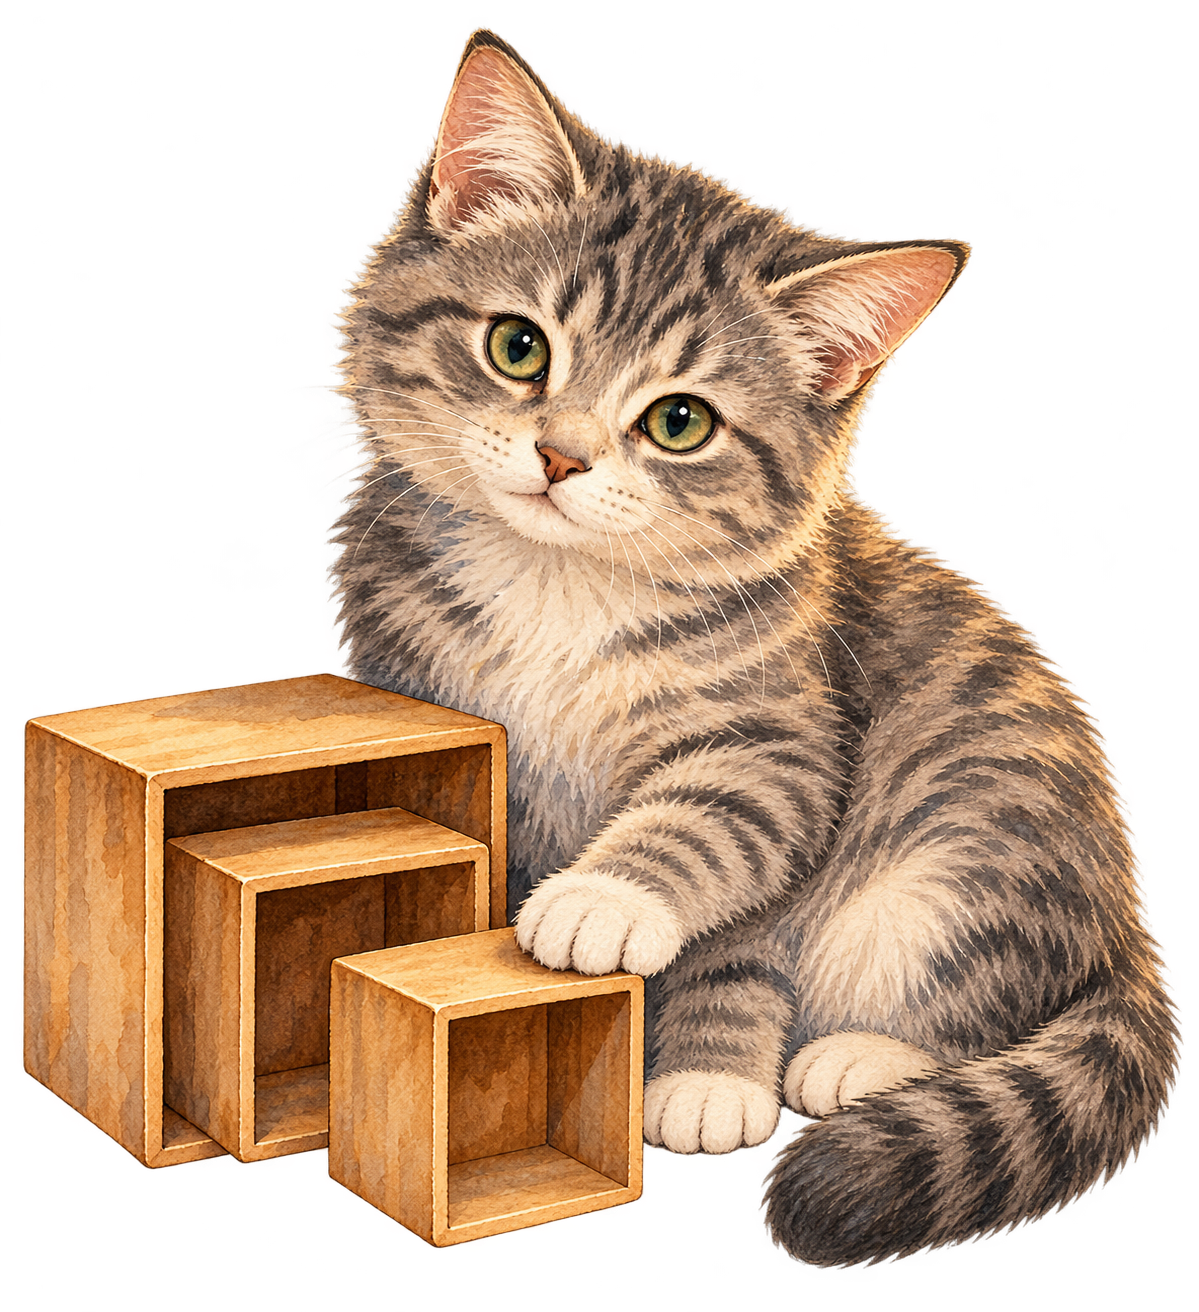
\includegraphics[width=54mm,height=58mm,keepaspectratio]{images/unique/art-11.png}
\end{wrapfigure}
\textbf{6.7.} Вычисли \((\dfrac{2}{3})^{- 2}\).\par

\textbf{6.8.} Вычисли \(10^{- 3} \cdot  10^{5}\).\par

\textbf{6.9.} Запиши \(0{,}00056\) в стандартном виде.\par

\textbf{6.10.} Запиши \(7{,}2 \cdot  10^{5}\) обычным числом.\par

\textbf{6.11.} Упрости \(a^{5} \cdot  a^{- 2}\) при \(a \ne  0\).\par

\textbf{6.12.} Вычисли \((- 2)^{3} \cdot  2^{- 2} + 3^{0}\).\par

\textbf{6.13.} Из жизни. В модели опыта каждая бактерия делится на две раз в час. Вначале была одна бактерия. Сколько их станет через \(8\) часов?\par
\par\WFclear\end{minipage}\end{lrbox}%
\ifdim\dimexpr\ht\CatFlowBox+\dp\CatFlowBox\relax<64mm\dp\CatFlowBox=\dimexpr64mm-\ht\CatFlowBox\relax\fi%
\noindent\usebox{\CatFlowBox}\par\addvspace{5pt}

\noindent\begin{minipage}[t]{\linewidth}\textbf{6.14.} Из жизни. Квадратный участок имеет сторону \(10^{3}\) м. Запиши его площадь степенью десяти и обычным числом в м\(^{2}\).\par\end{minipage}\par
\noindent\begin{minipage}[t]{\linewidth}\textbf{6.15.} Из жизни. В одном файле \(4 \cdot  10^{6}\) байт. Сколько байт в \(3 \cdot  10^{2}\) таких файлах?\par\end{minipage}\par
\noindent\begin{minipage}[t]{\linewidth}\textbf{6.16.}\starmark{} Вычисли: \(\dfrac{2^{- 3} \cdot  4^{2}}{8^{- 1}}\).\par\end{minipage}\par
\noindent\begin{minipage}[t]{\linewidth}\textbf{6.17.}\starmark{} Вычисли: \(\dfrac{3^{5} - 3^{4}}{3^{3} + 3^{2}}\).\par\end{minipage}\par
\noindent\begin{minipage}[t]{\linewidth}\textbf{6.18.}\starmark{} В модели файл каждый день увеличивается втрое. Через \(4\) дня его размер \(162\) МБ. Каков был размер сначала и каким станет через \(6\) дней от начала?\par\end{minipage}\par
\noindent\begin{minipage}[t]{\linewidth}\textbf{6.19.} Докажите, что \(a^m a^n=a^{m+n}\) для действительного \(a\) и натуральных \(m,n\), непосредственно используя определение натуральной степени.\par\end{minipage}\par
\noindent\begin{minipage}[t]{\linewidth}\textbf{6.20.} Пусть \(a\neq0\), \(m,n\) — натуральные числа. Докажите \(a^{-m}a^{-n}=a^{-(m+n)}\), используя определение отрицательной степени.\par\end{minipage}\par
\endgroup
